\chapter{Research Findings and Synthesis \label{ch:findings}}
\chaptertoc

This chapter presents and synthesizes the findings against the three research objectives. It first reports the cross-study evaluation results, then combines them with the findings of the five studies to answer the research questions.

\section{Results of the Cross-Study Evaluations\label{sec:cross_study_results}}

This section reports four cross-study evaluations in architecture recovery and C2A mapping. Boxplots pool 100 runs per method and system across all systems. They show the pooled distribution of outcomes without separating within-system from between-system variation. System-wise tests complement these plots.

\subsection{Recovery: Learning Objectives and Graph Inputs \label{sec:cont_recon}\label{sec:recovery_cross_study}}

The two recovery evaluations cover all fourteen benchmark systems. The first compares the contrastive approach of Paper~I with the reconstruction-based approach of Paper~II using GAT and common node features. It also includes GAT-E, the edge-attribute variant of Paper~I. The approaches retain their respective training settings, so the comparison does not isolate the learning objective alone.

The second compares the attributed-graph GCN and GAT of Paper~II with the structure-only methods of Paper~IV. These comprise GAT, GAT-DC, and N2V on the file-level dependency graph, and M2V and HGAT on the folder-augmented graph.

MoJoFM, ARI, and \cc{} measure agreement with the reference decomposition, while \tmq{} measures dependency cohesion independently of that reference. Figure~\ref{fig:overview-recovery} presents the results using MoJoFM and \tmq{}. The comparisons use a common clustering procedure, as described in Section~\ref{sec:cross_study_eval}.

\begin{figure}[!htb]
    \centering
    \begin{subfigure}{1\textwidth}
        \centering
        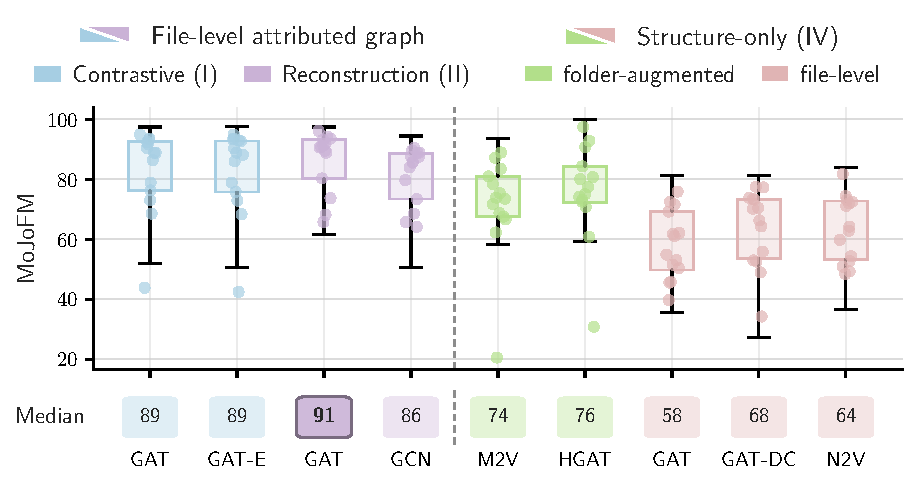
\includegraphics[width=1\textwidth]{figures/recovery_alignment.pdf}
         \caption{MoJoFM.}
        \label{fig:recovery-objectives}
    \end{subfigure}
    \par\vspace{0.3cm}
    \begin{subfigure}{1\textwidth}
        \centering
        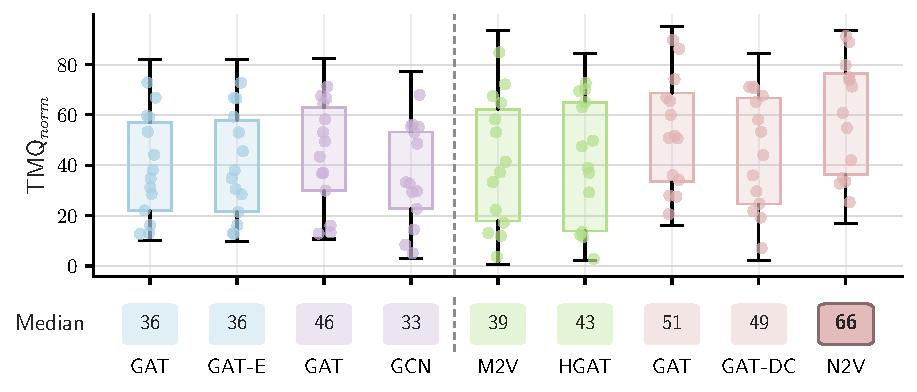
\includegraphics[width=1\textwidth]{figures/recovery_cohesion.pdf}
        \caption{Normalized TurboMQ (\tmq{}).}
        \label{fig:recovery-graphs}
    \end{subfigure}
    % \par
    \caption[Overview of recovery results across studies.]{Recovery results across studies: agreement with the reference decomposition (a) and dependency cohesion (b). The attributed-graph methods are the contrastive (Paper~I) and reconstruction (Paper~II) variants; the structure-only methods (Paper~IV) use the folder-augmented or the file-level graph. Boxplots pool all runs per system; dots mark system medians, and the boxed value indicates the median of these medians.}
    \label{fig:overview-recovery}
\end{figure}

\paragraph{Agreement with the reference decomposition.} In Figure~\ref{fig:overview-recovery}(a), the contrastive and reconstruction variants have similar median MoJoFM values, but the contrastive variants show a wider spread toward lower scores. System-wise comparisons significantly favor the reconstruction-based GAT over the contrastive GAT on both MoJoFM and ARI for nine of the fourteen systems. Effects are large for AS4, Bash, Chromium, Libxml, and OODT, and small to medium for C.Img, HDF, SH-3D, and TeamMates. Differences are not significant for ArgoUML, HDC, JabRef, or Lucene, while contrastive learning performs better only on Hadoop.

Adding edge attributes within the contrastive setup provides no consistent advantage. Mann--Whitney $U$ tests find a significant difference between GAT and GAT-E only for MoJoFM on OODT, with a small effect favoring GAT.

Comparing graph inputs, attributed GCN and GAT achieve a higher median MoJoFM than all structure-only methods. ARI and \cc{} give broadly similar rankings to MoJoFM when methods are ordered by their median scores across systems. The exceptions are that GCN ranks above the contrastive GAT variants under ARI, while GAT-DC and N2V exchange places under \cc{}.

\paragraph{Dependency cohesion.} Figure~\ref{fig:overview-recovery}(b) shows a different ordering from reference agreement. The file-level structure-only methods achieve higher median \tmq{} than the attributed methods, with N2V attaining the highest value. Among the attributed methods, reconstruction-based GAT scores above the contrastive variants, while GCN has the lowest median of all methods. Reconstruction-based GAT also scores above the folder-augmented HGAT and M2V.

Because \tmq{} varies widely across systems, we also compare each method with the reference architecture of the same system. Table~\ref{tab:gt_cohesion} reports how many systems have significantly lower or higher scores, using one-sample Wilcoxon signed-rank tests. GCN falls below the reference on eleven of fourteen systems. The contrastive and folder-augmented methods fall below it on seven or eight systems, whereas the remaining methods do so on five or fewer. N2V exceeds the reference on thirteen systems and falls below it only on Libxml.

Together, these comparisons show that agreement with the reference decomposition and dependency cohesion favor different methods. The attributed methods achieve higher reference agreement, while the file-level structure-only methods produce more dependency-cohesive partitions.

The common clustering procedure changes N2V's results relative to its original k-means configuration. Using Ward linkage lowers the median ARI across systems from 0.293 to 0.266 and MoJoFM from 68.9 to 63.5, while increasing normalized TurboMQ from 63.9 to 66.1. Changes in reference agreement vary in direction across systems, whereas normalized TurboMQ increases on thirteen of the fourteen systems.

\begin{table}[htb]
\centering
\caption[Recovered partitions compared with the ground truth in \tmq{}.]{Number of the fourteen systems on which a method's \tmq{} is significantly below or above that of the ground truth (one-sample Wilcoxon signed-rank test, $p<0.05$); on the remaining systems, the difference is not significant. \label{tab:gt_cohesion}}
\renewcommand{\arraystretch}{1.0}
\begin{adjustbox}{max width=\textwidth}
\begin{tabular}{@{} l cc cc cc ccc @{}}
\toprule
& \multicolumn{4}{c}{\textbf{Attributed graph (Papers~I \& II)}} & \multicolumn{5}{c}{\textbf{Structure-only (Paper~IV)}} \\
\cmidrule(lr){2-5}\cmidrule(lr){6-10}
& \multicolumn{2}{c}{Contrastive} & \multicolumn{2}{c}{Reconstruction} & \multicolumn{2}{c}{Folder-F} & \multicolumn{3}{c}{File-level} \\
\cmidrule(lr){2-3}\cmidrule(lr){4-5}\cmidrule(lr){6-7}\cmidrule(lr){8-10}
& GAT & GAT-E & GAT & GCN & M2V & HGAT & GAT & GAT-DC & N2V \\
\midrule
Below    & 8 & 8 & 5 & 11 & 8 & 7 & 2  & 5 & 1  \\
Above    & 4 & 4 & 7 & 3  & 6 & 5 & 11 & 9 & 13 \\
% Not sig. & 2 & 2 & 2 & 0  & 0 & 2 & 1  & 0 & 0  \\
\bottomrule
\end{tabular}
\end{adjustbox}
\end{table}

\subsection{Mapping: Predictors and Dependency Types \label{sec:mapping_cross_study}}

The two mapping evaluations cover the ten-system mapping benchmark and use macro- and micro-F1. The first compares HGT with the MLP, GCN, and GAT of Paper~III using the same file features and labeled sets. The graph-based predictors use a file-level graph with separate dependency relations.

The second compares typed and merged GAT using the four file representations from Paper~V. It examines whether the benefit of preserving dependency types extends beyond the combined lexical and folder-path features used in Paper~III.

\paragraph{Predictor comparison.} Figure~\ref{fig:overview-mapping} shows that GAT has the highest median macro- and micro-F1. HGT’s median micro-F1 lies between GCN and GAT, but its median macro-F1 is the lowest of all four predictors.
\begin{figure}[!htb]
    \centering
    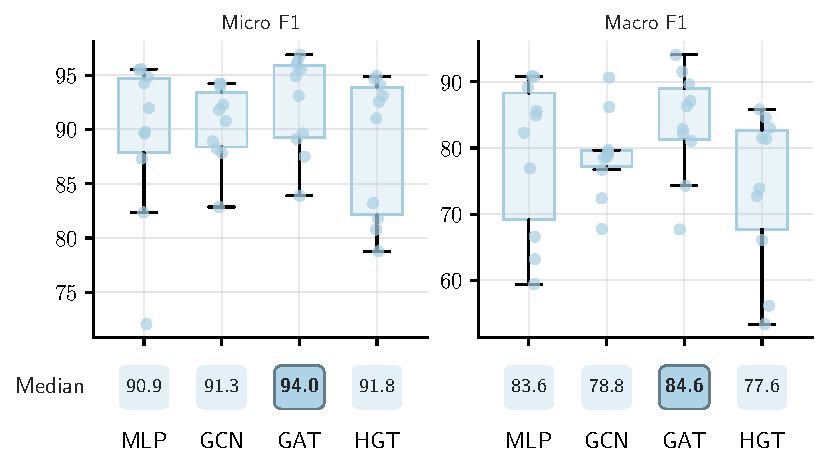
\includegraphics[width=0.90\textwidth]{figures/overview_mapping_benchmark.pdf}
    \caption[Overview of C2A mapping results across studies.]{Macro- and micro-F1 for MLP, GCN, GAT, and HGT on the same input features and labeled-set splits. Boxplots pool all runs per system; dots mark system medians, and the boxed value indicates the median of these medians.\label{fig:overview-mapping}}
\end{figure}

System-wise comparisons significantly favor GAT over HGT on nine of ten systems for macro-F1 and eight for micro-F1, with mostly large effects. HGT significantly outperforms GAT only on Chromium's micro-F1, by 1.9 points with a large effect.

HGT also generally performs worse than MLP and GCN. Compared with MLP, it scores significantly lower on seven systems for each metric, with small-to-large effects, and higher on Chromium and JabRef for both. Compared with GCN, it scores significantly lower on six systems for macro-F1 and five for micro-F1, and higher on two and four systems, respectively.

\paragraph{Effects of dependency type modeling.} Table~\ref{tab:gat_typed_summary} compares typed and merged GAT using Word2Vec, Node2Vec, and zero-shot (\zs{}) and fine-tuned (\ft{}) UniXcoder representations. Both variants use the GAT architecture of Paper~III with source-to-target aggregation. None of the input representations includes folder information.

Preserving dependency types yields positive median F1 differences across systems for all four representations. The largest median gain is for Word2Vec in macro-F1, at 5.8 points, and for fine-tuned UniXcoder in micro-F1, at 2.8 points. System-wise tests show significant gains on seven of ten systems for Word2Vec under both metrics, and on seven systems for fine-tuned UniXcoder in macro-F1 and nine in micro-F1.

The benefit is not uniform. Every representation also shows significant losses on some systems. Bash is a recurring exception, with significant losses for Word2Vec and both UniXcoder representations under both metrics. Zero-shot UniXcoder shows particularly mixed effects, with large gains on SweetHome-3D and HDF and large losses on Bash and Chromium.

\begin{table}[!htb]
\centering
\caption[Typed versus merged GAT across file representations.]{Typed minus merged GAT across ten systems. $\Delta$: median F1 difference (points); $+$ve: positive differences; $\uparrow$/$\downarrow$: significant gains/losses (paired Wilcoxon, Holm-corrected, $\alpha=0.05$). N/S/M/L: system counts by Cliff's $\delta$ magnitude (negligible/small/medium/large), regardless of direction or significance.}

\label{tab:gat_typed_summary}
\begin{adjustbox}{max width=\linewidth}
\renewcommand{\arraystretch}{1.2}
\begin{tabular}{l rcccc rcccc}
\toprule
& \multicolumn{5}{c}{Macro-F1}
& \multicolumn{5}{c}{Micro-F1} \\
\cmidrule(lr){2-6}\cmidrule(lr){7-11}
Vector
& $\Delta$ & $+$ve & $\uparrow$ & $\downarrow$ & N/S/M/L
& $\Delta$ & $+$ve & $\uparrow$ & $\downarrow$ & N/S/M/L \\
\midrule
N2V   & +0.6 & 6 & 5 & 1 & 5/4/0/1 & +0.8 & 7 & 7 & 3 & 4/4/0/2 \\
W2V   & +5.8 & 8 & 7 & 1 & 2/0/1/7 & +1.4 & 9 & 7 & 1 & 1/4/1/4 \\
\zs{} & +0.1 & 5 & 4 & 4 & 2/3/1/4 & +0.1 & 5 & 5 & 3 & 2/2/2/4 \\
\ft{} & +2.6 & 7 & 7 & 3 & 1/3/1/5 & +2.8 & 9 & 9 & 1 & 2/1/2/5 \\
\bottomrule
\end{tabular}
\end{adjustbox}
\end{table}
% % Requires \usepackage[table]{xcolor}
\begin{table*}[!htb]
\centering\small
\caption{Typed minus merged GAT per system, in F1 points: median over 100 paired splits, with the size of Cliff's $\delta$ (N/S/M/L) in parentheses. $^{*}$: significant (signed-rank, Holm across systems, $\alpha=0.05$). Shaded cells indicate significant negative differences.\label{tab:gat_typed_persystem}}
\begin{adjustbox}{max width=\textwidth}
\begin{tabular}{lrrrrrrrr}
\toprule
& \multicolumn{2}{c}{N2V} & \multicolumn{2}{c}{W2V} & \multicolumn{2}{c}{\zs{}} & \multicolumn{2}{c}{\ft{}} \\
\cmidrule(lr){2-3}\cmidrule(lr){4-5}\cmidrule(lr){6-7}\cmidrule(lr){8-9}
System & Macro & Micro & Macro & Micro & Macro & Micro & Macro & Micro \\
\midrule
A.UML & +1.7 (S)$^{*}$ & +0.9 (N)$^{*}$ & +1.3 (N) & +0.3 (N) & $-$0.4 (N) & +1.0 (S)$^{*}$ & +1.9 (S)$^{*}$ & +2.7 (M)$^{*}$ \\
C.Img & $-$0.3 (N) & +1.0 (S)$^{*}$ & 0.0 (N) & +1.4 (S)$^{*}$ & \cellcolor{gray!20}$-$2.8 (S)$^{*}$ & $-$1.4 (N) & \cellcolor{gray!20}$-$5.0 (L)$^{*}$ & +0.9 (N)$^{*}$ \\
JabRef & $-$0.3 (N) & \cellcolor{gray!20}$-$0.7 (S)$^{*}$ & +7.6 (L)$^{*}$ & +4.1 (L)$^{*}$ & +2.4 (S)$^{*}$ & +4.4 (L)$^{*}$ & +2.5 (S)$^{*}$ & +5.2 (L)$^{*}$ \\
Lucene & +0.9 (N)$^{*}$ & +0.3 (N)$^{*}$ & +3.9 (M)$^{*}$ & +0.9 (S)$^{*}$ & +0.6 (N) & \cellcolor{gray!20}$-$0.8 (S)$^{*}$ & +2.7 (M)$^{*}$ & +1.3 (M)$^{*}$ \\
SH-3D & $-$0.1 (N) & \cellcolor{gray!20}$-$1.5 (S)$^{*}$ & +5.8 (L)$^{*}$ & +1.5 (S) & +11.8 (L)$^{*}$ & +12.2 (L)$^{*}$ & +13.5 (L)$^{*}$ & +14.4 (L)$^{*}$ \\
T.Mates & \cellcolor{gray!20}$-$1.7 (S)$^{*}$ & \cellcolor{gray!20}$-$4.6 (L)$^{*}$ & +10.4 (L)$^{*}$ & +8.7 (L)$^{*}$ & +4.6 (M)$^{*}$ & +2.3 (M)$^{*}$ & +15.9 (L)$^{*}$ & +8.8 (L)$^{*}$ \\
Bash & +1.7 (S)$^{*}$ & +0.8 (N)$^{*}$ & \cellcolor{gray!20}$-$4.8 (L)$^{*}$ & \cellcolor{gray!20}$-$5.8 (L)$^{*}$ & \cellcolor{gray!20}$-$7.9 (L)$^{*}$ & \cellcolor{gray!20}$-$5.8 (L)$^{*}$ & \cellcolor{gray!20}$-$2.1 (S)$^{*}$ & \cellcolor{gray!20}$-$1.2 (N)$^{*}$ \\
HDF & +0.3 (N) & +2.5 (S)$^{*}$ & +9.8 (L)$^{*}$ & +13.9 (L)$^{*}$ & +5.6 (L)$^{*}$ & +4.1 (M)$^{*}$ & +7.4 (L)$^{*}$ & +7.3 (L)$^{*}$ \\
Chrome & +7.4 (L)$^{*}$ & +1.5 (L)$^{*}$ & +8.5 (L)$^{*}$ & +0.6 (S)$^{*}$ & \cellcolor{gray!20}$-$4.1 (L)$^{*}$ & \cellcolor{gray!20}$-$2.5 (L)$^{*}$ & +3.9 (L)$^{*}$ & +1.3 (L)$^{*}$ \\
HDC & +2.1 (S)$^{*}$ & +1.1 (N)$^{*}$ & +5.7 (L)$^{*}$ & +3.5 (M)$^{*}$ & \cellcolor{gray!20}$-$3.3 (S)$^{*}$ & $-$2.3 (N) & \cellcolor{gray!20}$-$0.5 (N)$^{*}$ & +2.9 (S)$^{*}$ \\
\bottomrule
\end{tabular}
\end{adjustbox}
\end{table*}
% _________ Contrubutions __________________
\section{Synthesis of Research Findings \label{sec:contruibutions}}

This section combines the findings of the five studies with the cross-study results in Section~\ref{sec:cross_study_results} to answer the research questions. The synthesis follows the three research objectives, examining the use of representation learning for recovery and mapping, the information carried by individual implementation signals, and the contribution of additional graph structure.

% ===== OBJECTIVE 1 Answers START ===========
\subsection{Objective~1: Representation Learning for Recovery and Mapping\label{sec:cont_1}}

Objective~1 examines how graph-based representation learning supports architecture recovery and C2A mapping. The findings address the combination of implementation signals (RQ1.1), the treatment of dependency types (RQ1.2), and the effects of learning objective, encoder architecture, and depth (RQ1.3).

\paragraph{RQ1.1: Combining implementation signals.} Papers~I--III combine dependencies, code identifiers, and folder organization to learn representations for recovery and mapping. These methods improve on their respective baselines in reference agreement for recovery and F1 for mapping. The results support the combined representations, but do not establish how much each signal contributes.

In Paper~III, a graph-free MLP using the same file features also outperforms the Naive Bayes baseline on every system under both F1 metrics. Improvement over that baseline therefore does not, by itself, demonstrate a benefit from dependency-based message passing.

\paragraph{RQ1.2: Modeling dependency types.} Papers~I--III represent dependency types as separate relations, each processed by its own encoder channel, and combine the outputs by summation. Paper~III compares this design with merging all dependencies into a single relation. With lexical and folder-token features, separate relations significantly improve both GCN and GAT across all evaluated systems. However, the separate channels also add parameters, so the comparison does not isolate dependency typing from model capacity. Papers I and II do not test a merged alternative.

The cross-study mapping comparison extends this evaluation to the folder-free representations of Paper~V. Separate relations generally benefit GAT, but the benefit is less consistent than in Paper~III and varies across representations and systems, with significant losses on some systems (Section~\ref{sec:mapping_cross_study}). HGT does not match GAT on the typed dependency graph, showing that the use of dependency types alone does not determine predictor performance.

Recovery provides less consistent support for separate relations. In Paper~IV, preliminary experiments on file-level dependency graphs showed markedly lower performance with separate relations, so the reported dependency-only comparisons use merged dependencies. With folder nodes and containment relations included, preserving dependency types gives modest benefits that vary across systems and evaluation measures.

Overall, separate dependency relations benefit mapping more consistently than recovery in the evaluated settings. Their effects vary with the input representations and encoder, but differences between the studies prevent these factors from being isolated.

\paragraph{RQ1.3: Learning objective, encoder architecture, and depth.} The studies examine how these three choices affect recovery and mapping.

\begin{itemize}[leftmargin=1em, topsep=3pt, itemsep=1pt]
\item \emph{Learning objective:} The cross-study evaluation in Section~\ref{sec:cont_recon} compares the contrastive approach of Paper~I with the reconstruction-based approach of Paper~II using common node features and a GAT encoder. Reconstruction generally achieves better agreement with the reference decomposition, although the advantage is not universal. Because the approaches retain different training settings, the comparison supports the reconstruction-based approach without isolating the learning objective alone.

\item \emph{Encoder architecture:} GAT generally outperforms GCN across recovery and mapping (Papers~II and~III), and HGT in the cross-study mapping comparison. GCN uses degree-normalized aggregation, whereas GAT learns weights for neighboring representations. However, the models also differ in parameterization, so these results cannot be attributed to attention alone. In mapping, GAT usually outperforms the graph-free MLP, while GCN frequently underperforms it. Access to dependencies therefore does not guarantee better predictions.

\item \emph{Encoder depth:} Paper~III finds no consistent benefit from increasing message-passing depth. A second layer improves performance on some systems and reduces it on others.
\end{itemize}

\begin{GrayBox}{Summary of Objective~1}
Combining dependency, lexical, and folder signals improves on the evaluated baselines in recovery and mapping, although the contribution of each signal is not isolated (RQ1.1). Preserving dependency types benefits mapping more consistently than recovery, with effects varying across inputs and encoders (RQ1.2). The reconstruction-based approach generally achieves better reference agreement than the contrastive approach, but their training settings also differ. GAT generally outperforms GCN across both tasks and HGT in the cross-study mapping comparison, while increasing encoder depth has no consistent benefit (RQ1.3).
\end{GrayBox}
% _________ Objective~2 __________________

\subsection[Objective~2: Architectural Information in Implementation]{Objective~2: Architectural Information in Implementation Signals \label{sec:cont_2}}

Objective~2 (Sec.~\ref{sec:obj_2}) examines the architectural information carried by individual implementation signals. The findings address recovery from dependency structure alone (RQ2.1), dependency-guided adaptation of contextual code representations (RQ2.2), and the comparison of structural, lexical, and contextual file representations (RQ2.3).

\paragraph{RQ2.1: Recovery from dependency structure.} Paper~IV shows that dependency structure alone supports recovery. N2V and GAT-DC outperform the classical recovery baselines, while plain GAT is generally weaker than both.

Structural reach helps explain this difference. N2V and GAT-DC achieve better reference agreement than the two-layer GAT on most systems. Applying diffusion to the GAT input graph closes much of the gap to N2V, suggesting that access to a wider dependency neighborhood contributes to recovery performance.

Performance also depends on how closely dependency structure follows the reference decomposition. Recovery is strongest when dependencies are concentrated within reference modules and remains difficult when within-module and cross-module dependencies are similarly dense, as on Hadoop and TeamMates.

The evaluation criterion matters as well (Section~\ref{sec:recovery_cross_study}). N2V produces the most dependency-cohesive partitions, while GAT-DC improves reference agreement over plain GAT on most systems without a corresponding advantage in dependency cohesion.

\paragraph{RQ2.2: Dependency-guided adaptation of code representations.} Paper~V finds that dependency-guided fine-tuning of UniXcoder improves mapping performance over its zero-shot form on nearly all systems. Both representations are held fixed during classifier training and evaluated using the same graph-free MLP and labeled sets, without folder information or additional message passing.

Fine-tuning uses a contrastive objective with positive pairs drawn mainly from two-hop dependency neighborhoods. This choice follows the observation in Paper~IV that structural context beyond direct neighbors can support recovery. With the classifier and evaluation conditions held fixed, the gains support adapting the pretrained representation to the target system using dependency information.

However, the comparison does not isolate the contribution of dependency-based pair selection, since it includes no fine-tuning alternative using pairs selected without dependency information.

\paragraph{RQ2.3: Comparing file representations.} Paper~V compares structural, lexical, and contextual file representations using the same graph-free MLP and labeled sets, without folder information or additional message passing. Representations that encode dependency information generally perform better. N2V captures dependencies through random walks, while \ft{} incorporates them through dependency-guided adaptation. Both generally outperform Word2Vec and \zs{}, although there are exceptions, including JabRef, where Word2Vec is among the strongest. Word2Vec and \zs{} show no consistent ordering, with each significantly outperforming the other on several systems.

Neither N2V nor \ft{} is uniformly best. N2V performs significantly better on six systems under both F1 metrics, while \ft{} performs significantly better on three systems under both metrics and additionally on HDC under macro-F1.

Together with the improvement from \zs{} to \ft{} (RQ2.2), these findings suggest that dependency information contributes to the stronger representations. However, the representations also differ in content and training procedure, so the contribution of dependency information alone cannot be isolated.

\begin{GrayBox}{Summary of Objective~2}
Dependency structure alone supports recovery, with performance depending on structural reach and how closely dependencies follow the reference modules. Reference agreement and dependency cohesion favor different methods (RQ2.1). Dependency-guided fine-tuning improves UniXcoder over its zero-shot form on nearly all systems, although the contribution of dependency-based pair selection is not isolated (RQ2.2). N2V and \ft{} generally outperform Word2Vec and \zs{} in mapping without folder information or additional message passing, but neither is uniformly best. Differences in content and training prevent the advantage from being attributed solely to dependency information (RQ2.3).
\end{GrayBox}

% % _________ Objective~3 __________________
\subsection[Objective~3: Interaction Between Input Signals and Graph]{Objective~3: Interaction Between Input Signals and Graph Structure \label{sec:cont_3}}

Objective~3 (Section~\ref{sec:obj_3}) examines how graph structure contributes beyond the initial file representations. The findings address dependency-neighbor aggregation and its direction (RQ3.1), folder organization (RQ3.2), and the additional detail provided by member nodes and edge attributes (RQ3.3).

\paragraph{RQ3.1: Dependency neighbors and aggregation direction.} Paper~V examines the contribution of dependency neighbors by enabling and disabling aggregation within HGT, GAT, and a neighbor MLP while holding file representations fixed. The neighbor MLP appends the mean of neighboring files' vectors to each file's own vector. These comparisons assess neighbor access within each predictor, avoiding the change in predictor architecture involved in comparing a GNN with a graph-free MLP.

Dependency neighbors improve mapping beyond the information already present in the file representations, but the gains vary across predictors and inputs. Gains are larger for Word2Vec and \zs{}, which do not encode dependencies, than for N2V. GAT is generally the strongest predictor, while HGT gains the least from neighbor access. With neighbors, \ft{} gains more than N2V, narrowing the gap observed without aggregation (RQ2.3).

Aggregation direction also affects performance. Source-to-target aggregation updates a file using information from files that depend on it, while undirected aggregation permits information to flow in both directions. The preferred direction varies across systems rather than across predictors or input representations. However, making the graph undirected also adds reverse edges, so the comparison does not separate direction from neighborhood size.

Paper~III examines aggregation direction for GAT and GCN and finds source-to-target aggregation generally preferable for GAT. This preference agrees with Paper~V on some systems but differs on others. The studies also differ in dependency typing, node features, depth, and training, so neither the benefit of aggregation nor the preferred direction can be assumed to transfer across settings.

These comparisons isolate neighbor access in mapping. The dependency-only recovery methods have no corresponding condition without dependency context. Their results instead show how recovery varies with structural reach and how closely dependencies follow reference-module boundaries (RQ2.1).

\paragraph{RQ3.2: Folder organization.} The studies represent folder organization either through directory tokens in file features (Papers~I--III) or through folder nodes and containment relations (Papers~IV and~V). In recovery, methods that include organizational information achieve better agreement with the reference decomposition, particularly where dependencies provide weak evidence of module boundaries. Dependency-only methods instead produce more dependency-cohesive partitions (Section~\ref{sec:recovery_cross_study}).

In mapping, Paper~V finds that adding folder nodes produces the largest and most consistent gains across the evaluated additions to the graph, with Word2Vec benefiting most. Across these configurations, folder nodes use the same folder-token features. With \ft{}, the folder-aware model approaches the mapping performance of a rule based on directory hierarchy and the initial labeled set on most systems, exceeding it only on Lucene.

The overall gains do not establish a consistent benefit for files whose directories are misleading. Among files misclassified by the directory-based rule, adding folder nodes and enabling message passing through them produces more corrections than regressions on some systems, but the reverse on others. Folder location is therefore informative for the reference mappings, while the model's ability to correct misleading directory assignments remains system-dependent. These mapping findings apply to HGT with source-to-target dependency aggregation.

\paragraph{RQ3.3: Member nodes and edge attributes.} Neither member-level nodes nor edge-level interaction attributes consistently improve performance in the evaluated settings.

In Paper~V, adding member nodes to the file-only graph lowers the median F1 for all three representations evaluated with HGT. When folder nodes are also present, the effect of adding member nodes varies with the representation. These additions change both the graph structure and how features enter the model, so their effects cannot be attributed to structure alone.

Paper~I reports small gains from edge attributes on some systems. However, the cross-study evaluation finds no significant improvement over the same model without these attributes (Section~\ref{sec:recovery_cross_study}). Paper~I attributes the limited benefit on TeamMates to edge attributes amplifying noisy cross-module interactions, suggesting that additional interaction detail may be less useful where dependencies poorly reflect module boundaries.

\begin{GrayBox}{Summary of Objective~3}
Dependency-neighbor aggregation improves mapping beyond the initial file representations, most reliably for GAT and the neighbor MLP. Gains vary across predictors and inputs, while the preferred aggregation direction varies across systems (RQ3.1). Folder organization provides the strongest additional signal in the evaluated mapping configurations, but does not consistently help correct files misclassified by the directory-based rule. In recovery, greater reference agreement can coincide with weaker dependency cohesion (RQ3.2). Adding finer-grained structure does not extend these benefits consistently. Member-level nodes give no consistent improvement in mapping, and edge-level attributes give no significant gain in the cross-study recovery evaluation (RQ3.3).
\end{GrayBox}

% Gains vary across predictors and inputs and narrow some of the differences between representations seen without aggregation, while the preferred aggregation direction varies across systems (RQ3.1).